\documentclass[landscape]{article}

\usepackage{2in1, lscape} 
\usepackage{units} 
\usepackage[fleqn]{amsmath}
\usepackage{float}
\usepackage{mdwlist}
\usepackage{booktabs}
\usepackage{caption}
\usepackage{fullpage}
\usepackage{enumerate}
\usepackage{graphicx}
\usepackage{parskip}
\usepackage{comment}

\everymath{\displaystyle}

\title{Crop Samples}
\date{\today}
\author{}

\excludecomment{note}

\begin{document}

  \maketitle
  % \tableofcontents
\begin{note}
  This information is from ``The Fascination of Statistics'', {\em
  Randomization, a historic controversy}.
\end{note}

  \section{Potatoes}

  \begin{table}[H]
    \centering
    \begin{tabular}{rrlrrl}
      \toprule
      Strip & Yield & Variety & Strip & Yield & Variety \\
      \midrule
      1     & 17.50 & C       & 11    & 17.50 & C \\
      2     & 18.00 & NC      & 12    & 20.50 & NC \\
      3     & 18.50 & C       & 13    & 15.50 & C \\
      4     & 15.50 & NC      & 14    & 16.00 & NC \\
      5     & 22.00 & C       & 15    & 17.50 & C \\
      6     & 16.50 & NC      & 16    & 16.50 & NC \\
      7     & 22.50 & C       & 17    & 14.50 & C \\
      8     & 15.50 & NC      & 18    & 11.50 & NC \\
      9     & 14.50 & C       & 19    & 16.00 & C \\
     10     & 14.50 & NC      & 20    & 13.00 & NC \\
      \bottomrule
    \end{tabular}
    \caption{Potato yields}
  \end{table}

  \begin{tabular}{lrr}
    \toprule
    variety & yield & sd \\
    \midrule
    C       & 17.60 & 5.54 \\
    NC      & 15.75 & 4.98 \\
     \bottomrule
  \end{tabular}

\begin{note}
  \paragraph{Notes}
  \begin{itemize*}
    \item $r = -0.5$. Each plot is -0.5 worse than the previous.
    \item Measured difference between C and NC\@: $\delta = 1.85$. Actual
      difference would be around $1.35$.
    \item Alternate design of (C, NC), (NC, C), (C, NC), etc. 
    \item Alternate design also plants on diagonal to previous planting to avoid
      some residual impact from planting.
  \end{itemize*}
\end{note}
  
  \begin{figure}[H]
    \centering
    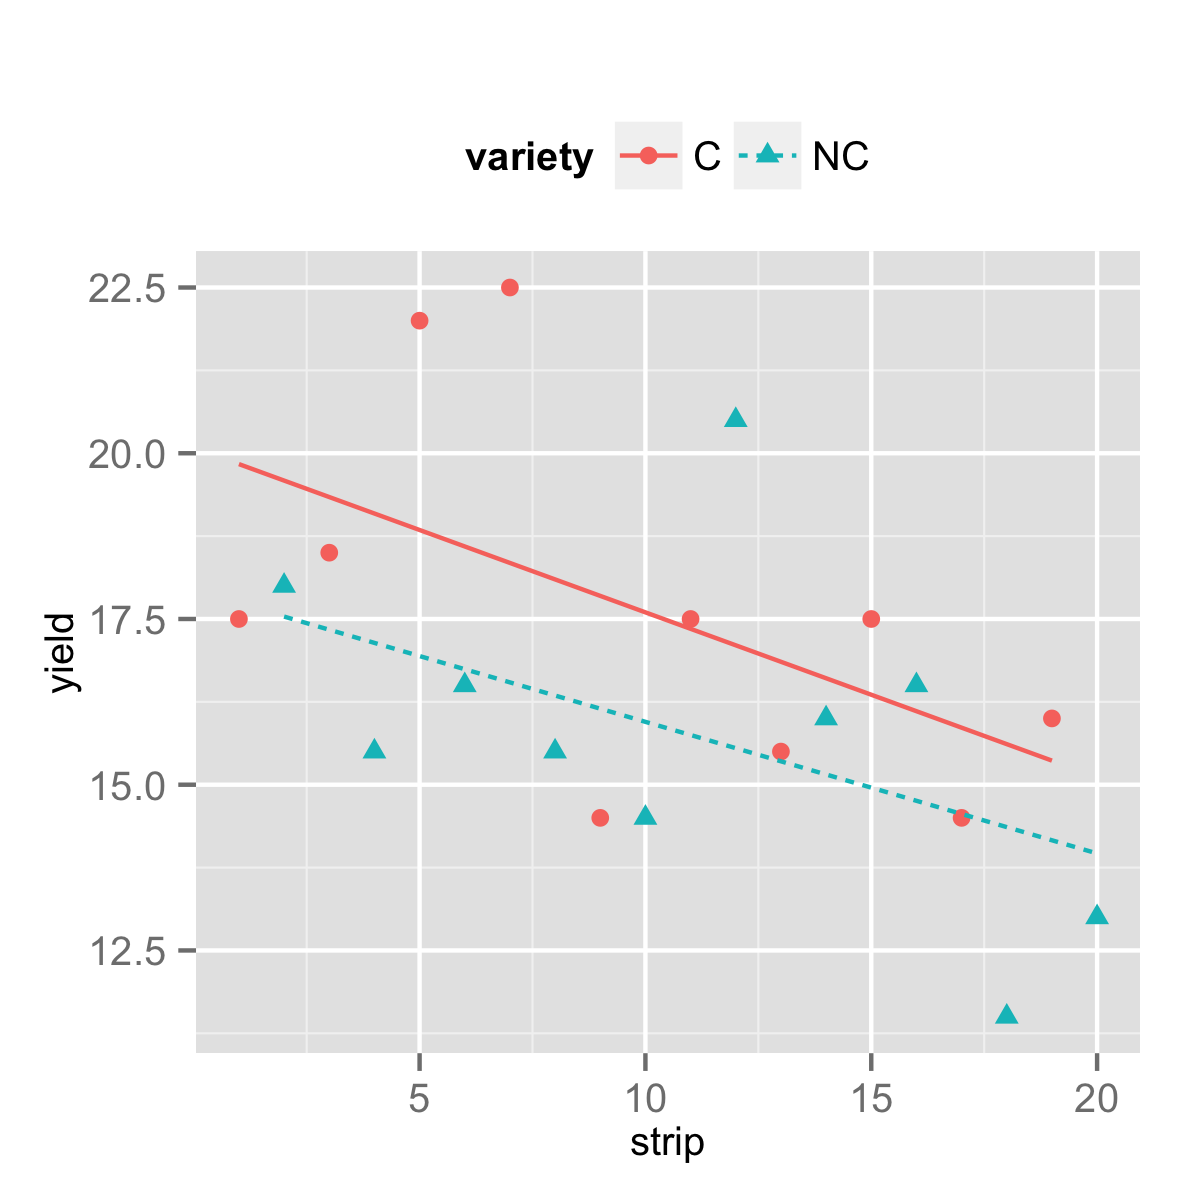
\includegraphics[width = 3in, height = 3in]{potatoes.png}
    \caption{Potato scatter plot}\label{fig:potatoes}
  \end{figure}

  \newpage

  \section{Imaginary Treatments} % (fold)

\begin{note}
  \paragraph{Notes}
  There were no actual treatment differences. The field was planted uniformly
  and then various imaginary treatments

  With a careful regular design, you can minimize the variation between
  treatments. Each treatment gets each part of the field. This is only possible
  if you can identify all the factors which might influence the outcome. This is
  possible with agriculture, but more difficult with, for example, human
  studies.

  The regular design tends to maximize the differences within each treatment.
  This is because every treatment is guaranteed to be present in the best part
  of the field (the left side in this case) and the worst side of the field (all
  the rest of the field). 

  With a careful regular design, the mean is likely to be correct, but the
  standard deviation for each treatment is likely to be large. With a random
  design, the mean is less likely to be correct, but the standard deviation
  within each group is likely to be smaller.

  To illustrate this, suppose 
  \begin{itemize*}
    \item the land gets 1 unit more productive with each slice
    \item treatment B is actually 2 units more productive than treatment A
    \item if field is laid out ABBAABBA, then the differences in each plot
      between B and A are 3, 1, 3, 1 for an average of 2 (correct) and standard
      deviation of 1.155 (max possible).
    \item if the decision of whether to put A or B first in each pair is random,
      it's likely that the differences will be either 3, 3, 3, 1 or 1, 1, 1, 3
      or something more extreme (all 1's or all 3's). With 3 matching values,
      the standard deviation is only 1, but the mean is either 2.5 or 1.5.
  \end{itemize*}

  With large numbers of plots, the difference between careful regular layout and
  random layout diminish.

  If you really can identify everything that may influence the outcome, you can
  get the most accurate estimate by accounting for everything, although this
  maximizes the apparent error in the estimate. If you can't identify everything
  that might influence the outcome, a simple random sample is the best choice.

\end{note}

  \begin{table}[ht]
    \centering
    \begin{tabular}{rllr}
      \toprule
      Plot & Regular & Random & Yield \\
      \midrule
      1    & A       & D      & 653 \\
      2    & B       & C      & 692 \\
      3    & C       & A      & 649 \\
      4    & D       & E      & 540 \\
      5    & E       & B      & 489 \\
      6    & F       & F      & 544 \\
      7    & A       & F      & 560 \\
      8    & B       & A      & 526 \\
      9    & C       & C      & 512 \\
      10   & D       & B      & 550 \\
      11   & E       & D      & 521 \\
      12   & F       & E      & 537 \\
      13   & F       & C      & 688 \\
      14   & E       & D      & 732 \\
      15   & D       & B      & 670 \\
      16   & C       & E      & 584 \\
      17   & B       & F      & 482 \\
      18   & A       & A      & 511 \\
      19   & F       & E      & 495 \\
      20   & E       & B      & 496 \\
      21   & D       & D      & 471 \\
      22   & C       & C      & 511 \\
      23   & B       & F      & 491 \\
      24   & A       & A      & 495 \\
      \bottomrule
    \end{tabular}
  \end{table}
  
  \begin{table}[ht]
    \centering
    \begin{tabular}{lrrr}
      \toprule
      Treatment & Mean & Delta & sd \\
      \midrule
      A       & 555        & -3     & 71 \\
      B       & 548        & -10    & 98 \\
      C       & 564        & 6      & 66 \\
      D       & 558        & 0      & 83 \\
      E       & 560        & 2      & 116 \\
      F       & 566        & 8      & 84 \\
      \midrule
      summary & (mean) 558 & (sd) 6 & (mean) 86 \\
      \bottomrule
    \end{tabular}
    \caption{Regular arrangement of plots.}
  \end{table}

  \begin{table}[ht]
    \centering
    \begin{tabular}{lrrr}
      \toprule
      Treatment & Mean & Delta & sd \\
      \midrule
      A       & 545        & -13     & 70 \\
      B       & 551        & -7      & 84 \\
      C       & 601        & 43      & 103 \\
      D       & 594        & 36      & 120 \\
      E       & 539        & -19     & 36 \\
      F       & 519        & -39     & 39 \\
      \midrule
      summary & (mean) 558 & (sd) 32 & (mean) 75 \\
      \bottomrule
    \end{tabular}
    \caption{Random arrangement of plots.}
  \end{table}
\end{document}

